
\chapter{Introduction}
\label{ch:INTR}
%\section{Section 1}
Autonomous vehicles are a class of vehicles that utilize multiple sensors such as LiDARs, RADARs, GPS-GNSS, cameras etc. to perceive its surroundings and move with scant or no human interaction \cite{kiran2021deep}. In the present world, lots of tasks are being automated to provide humans more convenience and safety. There can be scenarios where the drivers are not in a good state to drive, and it may lead to accidents. Instead, if the task of driving is given to an adequately trained machine, it will perform its task with maximum efficiency every single time. The web article \cite{grannyDLS} speaks about the evolution of autonomous vehicles. It states that the cars became autonomous first in 1920s and were called “Phantom Autos”. They were called so because they were remote controlled. Later in the 1980s self-managed autonomous cars were introduced by Mercedes, which were not fully automatic. It was performing lane change with human intervention. Because of the advancements in automobiles, information technology and the increasing interest in designing the autonomous cars by many young researchers, this will result in low-cost, reliable and efficient cars on the road in the near future.


\par
Autonomous driving systems consist of a few standard blocks as shown in Figure \ref{fig:fig1} \cite{kiran2021deep}. Scene understanding, localization, mapping, planning, driving policy and control are a few problems addressed by these modules. 

\begin{figure}[h]
	\centering
	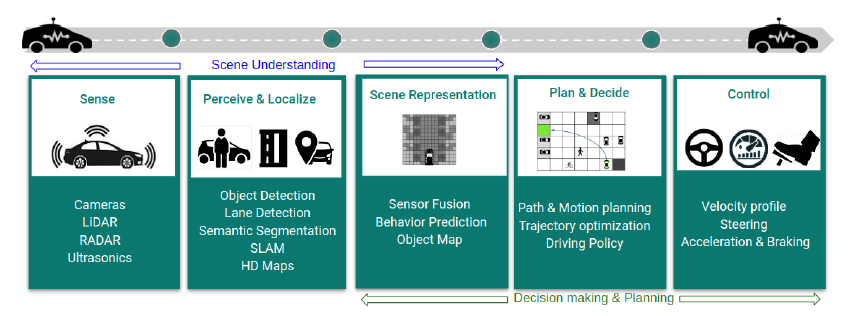
\includegraphics[width=1.0\textwidth]{fig1}
	\caption{Standard blocks of Autonomous Driving System \cite{kiran2021deep} }
	\label{fig:fig1}
\end{figure}


\par
Machine Learning (ML) models can be used to predict, classify/categorize and perform many more tasks. Usually, ML algorithms are classified into three broad categories: reinforcement, supervised and unsupervised learning. In supervised learning algorithms, the model is trained beforehand using labelled data to perform a certain task whereas in unsupervised learning the model is forced to learn from unlabelled data. Labelled data is a collection of information with one or more labels. These labels are useful tags with the help of which ML models can quickly interpret the data. Labelled data are the cornerstone of supervised learning \cite{fredriksson2020data}. The third category is Reinforcement Learning (RL) where an agent improves its performance in a task by constantly interacting with its surrounding. The classification and a few of its applications are as shown in Figure \ref{fig:fig0}. 

\begin{figure}[h]
	\centering
	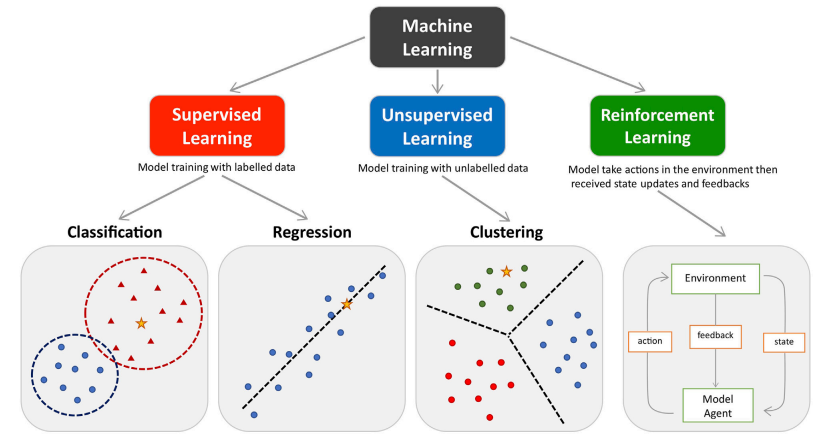
\includegraphics[width=1.0\textwidth]{ml_types}
	\caption{Classification of Machine Learning algorithms \cite{peng2021machine} }
	\label{fig:fig0}
\end{figure}

\par
For the process of autonomous driving which is a sequential decision problem, RL is the optimal choice as the vehicle needs to actively interact with its environment to drive safely. It is impossible to train the vehicle for all possible scenarios beforehand thus ruling out supervised and unsupervised learning approaches. There are a few challenges of using RL though, such as bridging the gap between simulation and reality, sample efficiency etc. Research in applying RL for autonomous driving requires tremendous effort from academicians, researchers and automotive industry experts from various fields to bring this idea into reality.

In the RL model, an autonomous agent masters its performance by persistent interaction with its environment. Reward function is a performance criteria which is used to evaluate the RL agent \cite{naveen2020survey}. The general scenario of RL is as shown in Figure \ref{fig:genRL}. At any time instance t, the agent in state $s_t$ which belongs to the state space S, chooses an action $a_t$ belonging to action space A and receives a reward $r_t \epsilon R$ (which can be positive or negative) from its environment based on the practicality of its decision. The agent then moves to the next state $s_{t+1}$ and proceeds to choose an action for this state. The cycle continues until the agent has learned the task completely or reached the final state. The agent’s objective is to maximize the cumulative rewards obtained during the entire lifetime of the task. Eventually, by exploiting the knowledge learnt, agent can increase the lifetime reward. It expands its knowledge by trial and error method \cite{naveen2020survey}. 



\begin{figure}
	\centering
	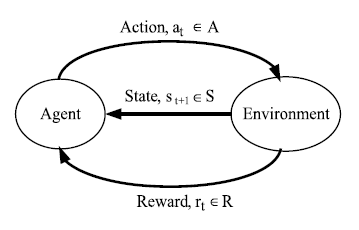
\includegraphics[width=0.6\textwidth]{fig2}
	\caption{General scenario of Reinforcement Learning \cite{naveen2020survey} }
	\label{fig:genRL}
\end{figure}



The prime challenge in RL is managing the balance between exploration and exploitation. To enhance the rewards it receives, an agent must exploit its knowledge by choosing actions that prove to be highly rewarding. In contrast, to ascertain such favourable actions, it has to make certain risky decisions. This may or may not result in higher rewards \cite{rahmati2019uw}. The strategy used by the agent to choose an action for a given state is known as a policy. If a particular policy gives maximum reward, such a policy is termed as optimal policy. 

RL can be used to solve many real world problems but sometimes, there exists certain situations where conventional RL algorithms fail to provide desirable resuls. This is mainly due to the fact that the state and/or action spaces involved in these problems are very high dimensional e.g. camera images, infrared images etc. and it is impossible to store all state- action pairs. To solve such problems, Deep Learning(DL) is used along with RL and it is referred to as Deep Reinforcement Learning(DRL). Usually, in DRL the policy is represented as a Neural Network. 

Deterministic Policy Gradient (DPG) is an algorithm that makes use of policy gradient function. Instead of representing the policy as a probability distribution, DPG uses gradient descent to create a policy that is deterministic in nature. The main advantage of DPG compared to other stochastic policy algorithms is that it is simpler and values can be computed more efficiently. But it comes with its own drawback, i.e. it becomes unstable when it it is used to solve problems with high dimensional state or action spaces. 

Conventional Q-learning algorithm calculates the Q values for state- action pairs and stores it in a tabular form. However, when the state and/or action spaces are very huge, it becomes infeasible to create table of Q values. Instead, neural networks are used as the memory and computation required would be less. Deep Q-Learning function approximator is used to solve such a problem. This learning algorithm is called Deep Q-Network (DQN). The primary advantage is that it can be used with high dimensional state and action spaces but it sometimes leads to over estimation of Q value due to random initialization of the same at the beginning. 




%Please include introduction about the project in this chapter.

%
%Introduction to the area of work (general discussion),  Brief present day scenario with regard to the work area
%
% Motivation, Shortcomings in the previous work / referenced paper,  Brief importance of the work in the present context,  Significance of the possible end result etc.
%
%Objectives
%
%Importance of the end result
%
%Organization of the project report (chapter wise)
%
%Electronic reference is given in \cite{sh07}. Journal article is given in \cite{odo95}. Article from conference is given in \cite{gs97}. Material from book \cite{cu72}. Manual detail is given in \cite{mo96}. Detail of technical report is given in \cite{jrc87}. A master thesis \cite{ka99} has been referred. A PhD thesis \cite{li2000} has been referred. Last referenec is taken from \cite{ro94}.
%\begin{definition}
%vvhffff
%\end{definition}
%
%\begin{figure}[bpht]
%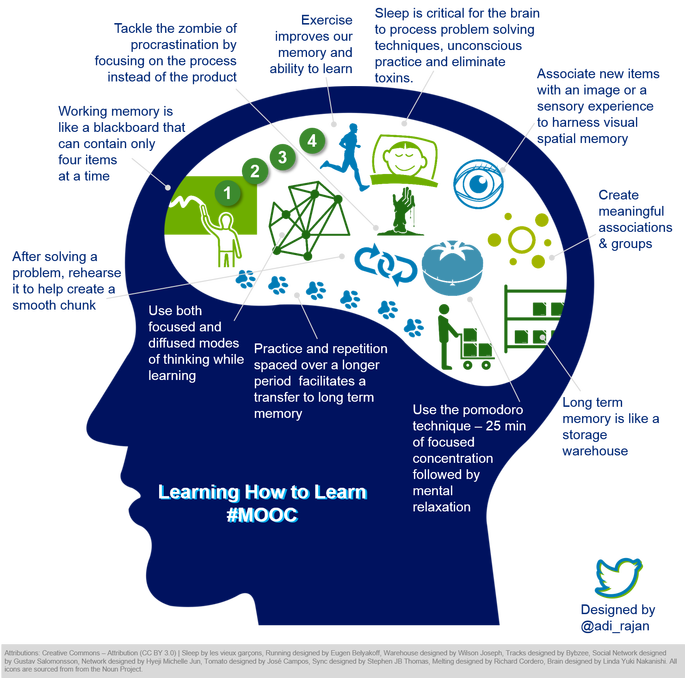
\includegraphics{Chapter1/LHTL}
%\caption{Learning how to learn}
%\end{figure}
%
%\begin{definition}
%fffffff
%\end{definition}
